\documentclass[tikz,border=4pt]{standalone}
\usepackage{amsmath}
\usepackage{xcolor}
\usetikzlibrary{arrows.meta,positioning,fit,calc}

\definecolor{ink}{HTML}{19232C}
\definecolor{subink}{HTML}{5B6872}
\definecolor{canvas}{HTML}{F8FAFC}
\definecolor{orange}{HTML}{D97706}
\definecolor{orangebg}{HTML}{FFF8F0}
\definecolor{green}{HTML}{168A50}
\definecolor{greenbg}{HTML}{F2FBF5}
\definecolor{blue}{HTML}{2767D4}
\definecolor{bluebg}{HTML}{F2F6FD}
\definecolor{red}{HTML}{D83C48}
\definecolor{purple}{HTML}{A45BD4}
\definecolor{grayedge}{HTML}{77838D}

\begin{document}
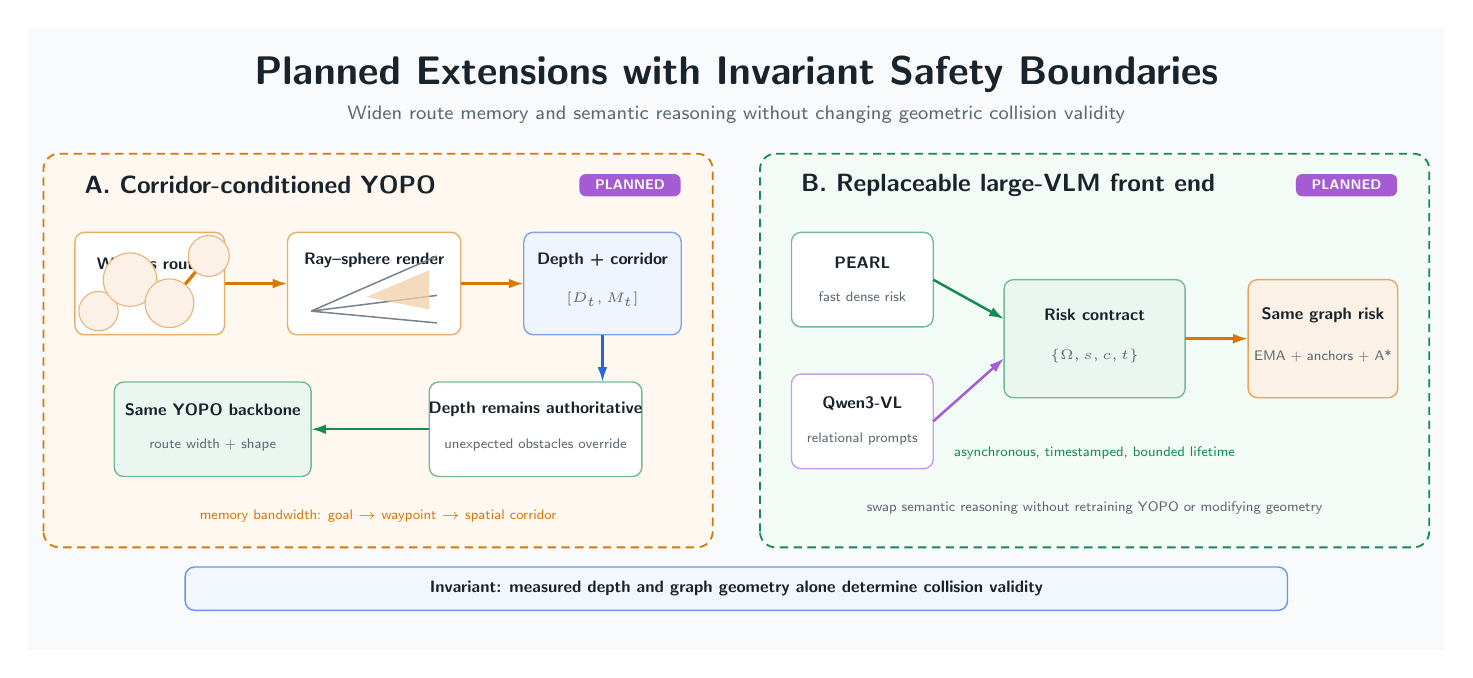
\begin{tikzpicture}[
  x=1mm,y=1mm,font=\sffamily,
  title/.style={font=\sffamily\bfseries\fontsize{14}{16}\selectfont,text=ink},
  subtitle/.style={font=\sffamily\fontsize{6.7}{8}\selectfont,text=subink},
  group/.style={font=\sffamily\bfseries\fontsize{9}{11}\selectfont,text=ink},
  nodetitle/.style={font=\sffamily\bfseries\fontsize{6.5}{8}\selectfont,text=ink,align=center},
  note/.style={font=\sffamily\fontsize{5.1}{6.4}\selectfont,text=subink,align=center},
  panel/.style={rounded corners=2mm,line width=.65pt,dashed,dash pattern=on 3pt off 2pt},
  box/.style={rounded corners=1.2mm,line width=.5pt,align=center},
  arrow/.style={-{Latex[length=1.9mm,width=1.25mm]},line width=.9pt,draw=grayedge},
  planned/.style={font=\sffamily\bfseries\fontsize{5.3}{6}\selectfont,text=white,fill=purple,rounded corners=.8mm,inner xsep=2mm,inner ysep=.8mm}
]
\fill[canvas] (-2,-5) rectangle (178,74);
\node[title] at (88,68) {Planned Extensions with Invariant Safety Boundaries};
\node[subtitle] at (88,63) {Widen route memory and semantic reasoning without changing geometric collision validity};

% Corridor extension
\filldraw[panel,fill=orangebg,draw=orange] (0,8) rectangle (85,58);
\node[group,anchor=west] at (4,54) {A. Corridor-conditioned YOPO};
\node[planned,anchor=east] at (81,54) {PLANNED};

\filldraw[box,fill=white,draw=orange!60] (4,35) rectangle (23,48);
\node[nodetitle] at (13.5,44) {Witness route};
\draw[orange,line width=1.2pt] (7,38)--(11,42)--(16,39)--(21,45);
\foreach \x/\y/\r in {7/38/2.5,11/42/3.4,16/39/3.1,21/45/2.6}{\draw[orange!55,fill=orange!10] (\x,\y) circle (\r mm);}

\filldraw[box,fill=white,draw=orange!60] (31,35) rectangle (53,48);
\node[nodetitle] at (42,44.5) {Ray--sphere render};
\draw[grayedge,line width=.55pt] (34,38)--(50,45) (34,38)--(50,40) (34,38)--(50,36.5);
\fill[orange!35,opacity=.75] (41,39.8)--(49,43.2)--(49,38.2)--cycle;

\filldraw[box,fill=blue!7,draw=blue!60] (61,35) rectangle (81,48);
\node[nodetitle] at (71,44.5) {Depth + corridor};
\node[note] at (71,39.5) {$[D_t,M_t]$};
\draw[arrow,draw=orange] (23,41.5)--(31,41.5);
\draw[arrow,draw=orange] (53,41.5)--(61,41.5);

\filldraw[box,fill=green!8,draw=green!60] (9,17) rectangle (34,29);
\node[nodetitle] at (21.5,25.5) {Same YOPO backbone};
\node[note] at (21.5,21) {route width + shape};
\filldraw[box,fill=white,draw=green!60] (49,17) rectangle (76,29);
\node[nodetitle] at (62.5,25.5) {Depth remains authoritative};
\node[note] at (62.5,21) {unexpected obstacles override};
\draw[arrow,draw=blue] (71,35)--(71,29);
\draw[arrow,draw=green] (49,23)--(34,23);
\node[note,text=orange] at (42.5,12) {memory bandwidth: goal $\rightarrow$ waypoint $\rightarrow$ spatial corridor};

% Qwen extension
\filldraw[panel,fill=greenbg,draw=green] (91,8) rectangle (176,58);
\node[group,anchor=west] at (95,54) {B. Replaceable large-VLM front end};
\node[planned,anchor=east] at (172,54) {PLANNED};

\filldraw[box,fill=white,draw=green!60] (95,36) rectangle (113,48);
\node[nodetitle] at (104,44.2) {PEARL};
\node[note] at (104,39.8) {fast dense risk};
\filldraw[box,fill=white,draw=purple!60] (95,18) rectangle (113,30);
\node[nodetitle] at (104,26.2) {Qwen3-VL};
\node[note] at (104,21.8) {relational prompts};

\filldraw[box,fill=green!8,draw=green!60] (122,27) rectangle (145,42);
\node[nodetitle] at (133.5,37.5) {Risk contract};
\node[note] at (133.5,32.3) {$\{\Omega,s,c,t\}$};
\draw[arrow,draw=green] (113,42)--(122,37);
\draw[arrow,draw=purple] (113,24)--(122,32);

\filldraw[box,fill=orange!10,draw=orange!65] (153,27) rectangle (172,42);
\node[nodetitle] at (162.5,37.5) {Same graph risk};
\node[note] at (162.5,32.3) {EMA + anchors + A*};
\draw[arrow,draw=orange] (145,34.5)--(153,34.5);

\node[note,text=green] at (133.5,20) {asynchronous, timestamped, bounded lifetime};
\node[note] at (133.5,13) {swap semantic reasoning without retraining YOPO or modifying geometry};

% shared invariant band
\filldraw[box,fill=bluebg,draw=blue!70] (18,0) rectangle (158,5.5);
\node[nodetitle] at (88,2.75) {Invariant: measured depth and graph geometry alone determine collision validity};
\end{tikzpicture}
\end{document}
